%!TEX root = ../notas_de_clase.tex

\section{Regresión No Lineal}
\label{sec:reg_no_lineal}

El modelo de regresión lineal visto en el capítulo anterior tiene diversas ventajas, en primer lugar su solución en el caso de mínimos cuadrados (o máxima verosimilitud en el caso de ruido gaussiano) puede ser encontrado de forma explícita y única. Además, sus parámetros permiten interpretar la relación entre cada una de las componentes de la variable de entrada y la variable de salida. Sin embargo, más allá de estas propiedades del modelo lineal, su alcance es muy limitado pues muchas veces necesitamos modelar fenómenos que no siguen una relación lineal. 

El concepto de regresión lineal puede ser extendido a una contraparte no lineal en los casos particulares que conocemos a priori el tipo de relación entre las variables de entrada $x$ y salida $y$ (y esta  no es lineal). Dicha extensión puede ser obtenida simplemente mediante la aplicación de una transformación (de parámetros fijos) a la variable independiente, e.g. $\phi(x)$, para luego construir un modelo lineal en la variable transformada $\phi=\phi(x)$ en lugar de en la variable original $x$. 

Específicamente, consideraremos transformaciones a valores vectoriales de la variable independiente de la siguiente forma
\begin{align}
  \phi \colon \R^M &\to \R^D \nonumber\\
  x &\mapsto \phi(x)=[\phi_1(x),\ldots,\phi_D(x)]^\top,
\end{align}
donde $\phi_i: x\in\R^M \mapsto \phi_i(x)\in\R, \forall i=1,\ldots,D$ son funciones escalares. 

Con la introducción de la transformación $\phi(\cdot)$ es necesario hacer la distinción entre ambas variables de entrada. Nos referiremos entonces a $x$ como datos/entradas crudos (\emph{raw data/input}) y a la variable  $\phi=\phi(x)$ como  características (\emph{features}). Recordemos que los modelos del capítulo anterior eran aplicados directamente sobre la entrada cruda $x$ (o $\tilde{x}$), con lo que no existía distinción entre entradas crudas o características. Adicionalmente, la introducción  del concepto de \emph{característica} es motivado por la búsqueda de una representación de $x$ que permite resolver el problema de regresión usando un modelo de simple (y también interpretable) como el modelo lineal, esto está en contraste con la idea de diseñar un modelo muy complicado (no interpretable) que reciba directamente la entrada cruda $x$. Un ejemplo de esto es el caso en que $x$ es una imagen: en este caso no es posible aplicar directamente un modelo lineal a la representación matricial de la imagen, sino que a una representación distinta de este, o a sus \emph{características}, es decir, sus bordes, formas, y otros patrones a identificar dentro de la imagen. 

En la práctica, la función $\phi:x\mapsto\phi(x)$ es elegida en base  al conocimiento \emph{experto} que se tenga del problema de regresión a resolver;  como su elección pretende extraer las características de interés y representarlas  de una forma compatible con el modelo lineal, entonces, nos referiremos a la construcción \emph{manual} de la función $\phi$ como \emph{ingeniería de características}. Observemos entonces que la función $\phi$ puede tener (y en general tiene) parámetros, los cuales en esta primera instancia serán elegidos manualmente. Sin embargo, más adelante veremos modelos donde los parámetros de $\phi$ también pueden ser encontrados de forma automática (e.g., mediante máxima verosimilitud). En dicho caso, es posible interpretar que la ingeniería de características ya no es realizada de forma manual, sino que automatizada.  



\begin{mdframed}[style=discusion, frametitle={\center Características y modelos}]
El diseño de características es uno de los problemas fundamentales del AM. Esto porque podemos entender la construcción de modelos de aprendizaje supervisado como dos etapas: i) la identificación de las características relevantes y ii) cómo usar estas características para estimar el output (el modelo). En el modelo no lineal presentado aquí, es claro que la parte no lineal $\phi$ es la característica y la parte lineal es el modelo, sin embargo, en el caso general la línea entre ambas etapas es muy delgada.  Por ejemplo, en una red neuronal de 100 capas, ¿qué corresponde a característica y qué corresponde al modelo? Podríamos argumentar que en modelos más complicados como los de redes neuronales, existen varias interpretaciones de qué corresponde a cada cosa, y con eso de paso interpretar qué está haciendo nuestro modelo. El hecho de que el diseño de características y el modelo se confundan es interesante también, pues quiere decir que las características se aprenden de igual forma que el resto del modelo; con lo que pasamos desde un diseño manual de características a una búsqueda automáticas de características. 

\end{mdframed}


\subsection{Modelo lineal en los parámetros} 
\label{sub:modelo_lineal_param}


Usando la nueva variable de  características $\phi=\phi(x)$ como entrada a un modelo lineal, podemos definir el siguiente modelo de regresión lineal y gaussiano: 
\begin{equation}
    y = \theta^\top\phi(x) + \epsilon,\quad \epsilon\sim\cN(0,\sigma_\epsilon^2)\label{eq:reg_no_lin},
\end{equation}
donde asumiremos que contamos con un conjunto de observaciones de la forma
\begin{equation}
    \datos = \{(x_i,y_i)\}_{i=1}^N,\quad (x_i, y_i)\in\R^M\times\R^1,\forall i=1,\ldots,N.
    \label{eq:training_set_nl}
\end{equation}

De la misma forma que vimos en el capítulo anterior, este modelo puede ser entrenado mediante el la optimización de costo cuadrático
\begin{align}
    J &= \frac{1}{2} \sum_{i=1}^N(y_i - \theta^\top\phi(x_i))^2,
\end{align}
lo cual es equivalente a máxima verosimilitud, pues el ruido de observación $\epsilon$ es gaussiano.

Para una presentación sencilla, evitaremos el uso de las sumatorias y adoptaremos la siguiente notación matricial:
\begin{align}
    X = \left[ \begin{matrix} x_1 \\ \vdots \\ x_N \end{matrix} \right]\qquad
    \Phi = 
    \left[ \begin{matrix} \phi(x_1)\\
    \vdots \\
    \phi(x_N)\\
    \end{matrix} \right]
     = \left[ \begin{matrix} \phi_1(x_1)& \ldots & \phi_D(x_1)\\
    \vdots & \ddots & \vdots \\
    \phi_1(x_N) & \ldots & \phi_D(x_N)\\
    \end{matrix} \right]
    \qquad
    Y = \left[ \begin{matrix} y_1 \\ \vdots \\ y_N \end{matrix} \right],
\end{align}
con lo que el modelo y el funcional de costo puede ser expresados respectivamente mediante
\begin{align}
    Y &= \Phi\theta + \bepsilon,\quad \bepsilon\sim\cN(\mathbf{0},\sigma_\epsilon^2\mathbf{I})\\
    J &= \frac{1}{2} (Y-\Phi\theta)^\top(Y-\Phi\theta).
\end{align}

De forma análoga al modelo lineal estándar (el cual toma directamente la variable cruda $x$ como input), la minimización del funcional $J$ puede  ser encontrado mediante la condición de primer orden $\nabla_\theta J=0$ y está dada por 
\begin{align}
    \theta{\star}&= (\Phi^\top\Phi)^{-1}\Phi^\top Y\label{eq:nolin_theta}.
\end{align}
Las siguientes observaciones conectan el modelo no lineal de la ec.~\eqref{eq:reg_no_lin} con el modelo lineal estudiado en el Capítulo \ref{cap:reg_lineal}.


\begin{remark}
De la ec.~\eqref{eq:nolin_theta} vemos que si elegimos $\phi(\cdot) = \text{id}(\cdot)$ recuperamos la expresión para mínimos cuadrados ordinarios. Esto permite interpretar el modelo de regresión no lineal con variables $\{(x_i,y_i)\}_{i=1}^N$ de $\R^N$ a $\R$ como una regresión lineal con variables $\{(\Phi(x_i),y_i)\}_{i=1}^N$ de $\R^D$ a $\R$. Además, la razón por la que la forma de la solución es la misma que el caso lineal es porque si bien el modelo presentado en la ec.~\eqref{eq:reg_no_lin} es no  lineal en la entrada $x$, este es \emph{lineal en los parámetros} $\theta$.
\end{remark}

\begin{remark}
Notemos que la re-parametrización del modelo afín introducida en el capítulo anterior es un caso particular de la transformación $\Phi$. Esto es directo de la siguiente construcción:
\begin{align*}
    \Phi &= [x, 1]^\top\\
    y &= a^\top x + b  =  \theta^\top\Phi(x)+ \epsilon.
\end{align*}
\end{remark}


\begin{remark}
    Finalmente, es posible considerar una extensión regularizada al modelo no lineal presentado en la   ec.~\eqref{eq:reg_no_lin} mediante la consideración de un costo regularizado cuadrático (i.e., \emph{ridge regression}) dado por 
\begin{equation}
    J_r = \frac{1}{2} \sum_{i=1}^N(y_i - \phi(x_i)\theta)^2 + \rho\left \| \theta \right \|^2,\quad \rho\in\R^+.
\end{equation}
En cuyo caso, la solución está dada por
\begin{equation}
    \theta = (\Phi^\top\Phi+\rho\mathbb{I})^{-1}\Phi^\top Y.
\end{equation}
\end{remark}


\begin{mdframed}[style=discusion, frametitle={\center (S)elección de características}]

Un buen conjunto de características no solo ayuda a una buena representación (y consecuentemente predicción) de nuestros datos, sino que extrae literalmente las  \emph{características} que son relevantes de $x$ para determinar $y$. Por ejemplo, si necesitamos determinar la condición clínica de un  paciente, para el cual tenemos una vasta colección de  mediciones como peso, edad, género, dirección, número de teléfono, ocupación, color de ojos, salario, etc, muy probablemente muchas estas características no van a ser útil (por ejemplo, ocupación), con lo que el diseño de las funciones $\phi$ debe tomar en cuenta esto. Por el contrario, si necesitamos evaluar el mismo conjunto de individuos  para un crédito de consumo, las características a considerar variarán y ahora probablemente el salario sí juegue un rol importante. Este concepto permite entender la estrecha relación entre el diseño de características y la \emph{selección de características} y consecuentemente la \emph{selección de modelos}, lo cual veremos en los siguientes capítulos. En particular, recordemos que usando el regulador LASSO, podemos llevar algunas de nuestras coordenadas a cero, realizando una selección automática de características. 

\end{mdframed}




\subsection{Ejemplos de transformaciones}

La selección de las características es fundamental para una representación apropiada de nuestros datos y consecuentemente para el desempeño del modelo de regresión no lineal. En efecto, si la familia de funciones $\phi_1,\ldots,\phi_D$ no captura la representación de las características de forma compatible con el modelo lineal, el esfuerzo por ajustar la parte lineal del modelo será infructuoso. En general, la elección de la base de funciones debe ser diseñada y evaluada caso a caso.\\

A continuación vemos algunos ejemplos de características que son usualmente usadas en la práctica por su generalidad (habilidad para replicar varios comportamientos) y/o simpleza.\\

\noindent\textbf{Función Polinomial:} $\phi=\{\phi_i\}_{i=0}^D$, donde $\phi_i(x)=x^i$, de tal forma que 
\begin{equation}
    \Phi = \left[ \begin{matrix} 1 & x_1 & x_1^2 & \ldots & x_1^D\\
    \vdots & \vdots & \vdots & \ddots & \vdots \\
    1 & x_N & x_N^2 & \ldots & x_N^D\\
    \end{matrix} \right].
\end{equation}
La función polinomial es ampliamente usada debido sla capacidad de la base polinomial para aproximar cualquier función \emph{bien portada} con una precisión determinada (considerando un grado  $D$ suficientemente  grande). Sin embargo, una desventaja de esta  base es que tanto su entrenamiento como  predicciones pueden ser inestables: si se usa un grado $D$ muy alto,  los valores de $\phi(x)$ crecen, obviamente, de forma \emph{polinomial}.\\

\noindent\textbf{Función Sinusoidal:} $\phi=\{\phi_i\}_{i=0}^D$, donde $\phi_i(x)=\cos\left(i\frac{2\pi}{2T}(x - b_i)\right)$. La variable $i$ actúa como una frecuencia normalizada con respecto al período de oscilación $T$ y $b_i$ es un ``offset''  o fase. Esta transformación está dada por
\begin{equation}
    \Phi = \left[ \begin{matrix}
    1 & \cos\left(1\frac{2\pi}{2T}(x_1-b_1)\right) & \ldots & \cos\left(D\frac{2\pi}{2T}(x_1-b_D)\right)\\
    \vdots & \vdots  & \ddots & \vdots \\
    1 & \cos\left(1\frac{2\pi}{2T}(x_N-b_1)\right) & \ldots & \cos\left(D\frac{2\pi}{2T}(x_N-b_D)\right)\\
    \end{matrix} \right].
\end{equation}
Hemos asumido que el la fase para cada función $\phi_i$, la frecuencia $i\frac{2\pi}{2T}$ y fase $b_i$ son fijas. Una forma de evitar definir una fase, es considerar dos transformaciones por cada $\phi_i$ de la forma
\begin{equation}
    \phi_i'(x) = \left[\sin\left(i\frac{2\pi}{2T}x\right),\ \cos\left(i\frac{2\pi}{2T}x\right)\right],
\end{equation}
donde no es necesario definir la fase sino que ésta es absorbida por el parámetro $\theta$ y aprendida.  

Al igual que los polinomios, la base de cosenos es también \emph{universal}. Sin embargo, una desventaja de la base senoidal es que solo puede replicar funciones periódicas, con un período máximo en este caso  de $T$. En la práctica, veremos que un modelo sinusoidal se repetirá cada período, pudiendo llevar a conclusiones erróneas. Además, si efectivamente nuestros datos representan un comportamiento periódico pero el ruido de observación resulta en que cada período o \emph{forma de onda} sean ligeramente distinto, puede ser difícil encontrar el período $T$. La identificación de este período es un desafío en sí mismo, conocido como \emph{detección de periodicidades o frecuencias fundamentales}, usual en astronomía y procesamiento de audio. \\

\noindent\textbf{Funciones constantes por partes:} La siguiente característica está está compuesta por ``escalones'', los cuales valen ``1'' dentro de un conjunto especifico y ``0'' en cualquier otro lugar. Sean $c_1,c_2, \ldots,c_D\in\R$ una colección de valores crecientes, definimos la indicatriz $I_A$ y las funciones de pertenencia $C_i$:
\begin{align}
    C_0(x) &= I_{(-\infty,c_1)}(x)\\
    C_i(x) &= I_{[c_i,c_{i+1})}(x), \quad \forall i=1,\ldots,D-1\\
    C_D(x) &= I_{[c_D,+\infty)}(x)\\
    I_A(x) &= \left\{\begin{matrix}
    1,\quad x\in A\\
    0,\quad x\notin A
    \end{matrix}\right. 
\end{align}
De esta forma la base de funciones $\Phi=\{\phi_i\}_{i=0}^D$ queda definida por
    
\begin{align}
    \phi_i(x) &= C_i(x),\quad \forall i=0,\ldots,D\\
    \Phi(X) &= \left[ \begin{matrix}
    1 & C_0(x_1) & \ldots & C_D(x_1)\\
    \vdots & \vdots  & \ddots & \vdots \\
    1 & C_0(x_N) & \ldots & C_D(x_N)\\
    \end{matrix} \right].
\end{align}
Las funciones contantes por partes son útiles cuando trabajamos con experimentos que involucran una discretización, por ejemplo, al modelar la altura/concentración/conductividad/temperatura en una superficie y no es posible parametrizar esta cantidad como función del (en este caso) espacio. Entonces, simplemente dividimos la superficie en una grilla y asignamos un valor distinto a cada celda de esta grilla. Es un método útil pero la cantidad de parámetros (dimensión de $\theta$) crece con el número de celdas de la grilla, lo cual es prohibitivo para casos donde el  rango de valores de $x$ y/o su dimensión es medianamente alta. 
    
\iffalse
\noindent\textbf{Polinomios por partes (Splines)}: Una generalización de las funciones constantes por partes es ajustar polinomios truncados definidos en intervalos. Es decir, podríamos considerar el siguiente modelo truncado (dos partes solamente) 
\begin{equation}
    y = \left\{\begin{matrix}
    \beta_{01}+\beta_{11}x+\beta_{21}x^2+\beta_{31}x^3+\epsilon,\quad x < c\\
    \beta_{02}+\beta_{12}x+\beta_{22}x^2+\beta_{32}x^3+\epsilon,\quad x \geq c
    \end{matrix}\right.
\end{equation}
    
El problema con esta formulación es que en el punto $c$ no existe ninguna restricción de continuidad, lo cual es muchas veces necesario para que el modelo tenga sentido y refleje la realidad. Podemos arreglar esta discontinuidad de la siguiente forma.

Consideremos una secuencia de puntos crecientes $\xi_1,\ldots,\xi_K$ que serán los puntos en que cambia el régimen del polinomio, estos puntos se conocen como \emph{nudos}; en el ejemplo anterior solo consideramos un nudo para ilustrar. Podemos ahora definir el un polinomio truncado de grado $i$ con un nudo en $\xi_k$ mediante
\begin{equation}
    (x-\xi_k)_+^i = \left\{\begin{matrix}
    0,\quad x < \xi_k\\
    (x-\xi_k)^i,\quad x \geq \xi_k
    \end{matrix}\right.
\end{equation}
Con esto polinomio truncado de grado $D$ y con $K$ nudos queda definido por
    
    \begin{equation}
        y = \beta_0 + \sum_{d=1}^D\beta_dx^d+\sum_{k=1}^K(x-\xi_k)_+^D
    \end{equation}
    
    \begin{equation}
        \Phi(X) = \left[ \begin{matrix} 1 & x_1 & x_1^2 & \ldots & x_1^D & \ldots & (x_1-\xi_1)_+^D & \ldots & (x_1-\xi_K)_+^D \\
        \vdots & \vdots & \vdots & \ddots & \vdots & \ddots & \vdots & \ddots & \vdots\\
        1 & x_N & x_N^2 & \ldots & x_N^D & \ldots & (x_N-\xi_1)_+^D & \ldots & (x_N-\xi_K)_+^D \\
        \end{matrix} \right]
    \end{equation}

\fi


\begin{mdframed}[style=ejemplo, frametitle={\center Ejemplo: Predicción de pasajeros de una aerolínea)}]

Consideremos el problema de predecir la cantidad de pasajeros en una aerolínea, considerando  distintas combinaciones de características. De forma incremental, tomaremos en consideración características polinomiales,  senoidales, y senoidales con amplitud creciente. Es decir, denotando $x$ en tiempo y $y$  la cantidad de pasajero, consideraremos el siguiente modelo
\begin{equation}
    y = \underbrace{\sum_{i=0}^3 \theta_i x^i}_\text{parte polinomial} + \underbrace{ \sum_{i=1}^2 \alpha_i\exp(-\tau_ix^2)\cos(\omega_i(x-\psi_i))}_\text{parte oscilatoria}.
\end{equation}
La motivación de este modelo es representar la tendencia de los datos mediante la componente polinomial y la oscilación anual mediante las componentes oscilatorias.

Además, hemos considerado 12 años de datos con frecuencia mensual (144 datos), de los cuales solo 9 años (108 datos) han sido usado para encontrar los parámetros del modelo y los  3 años restantes (36 datos) para validar nuestras predicciones. La Figura \ref{fig:pasajeros} muestra los datos y las estimaciones para 3 variantes del modelo mencionado: parte polinomial, parte polinomial y oscilatoria de amplitud fija, y finalmente,  parte polinomial y oscilatoria de amplitud variable. En cada gráfico se muestran distintas opciones de cada  modelo en gris con la mejor  trayectoria en negro; se puede ver además en cada gráfico cómo disminuye el error de aproximación a medida consideramos más características. 


\begin{figure}[H]
    \centering
    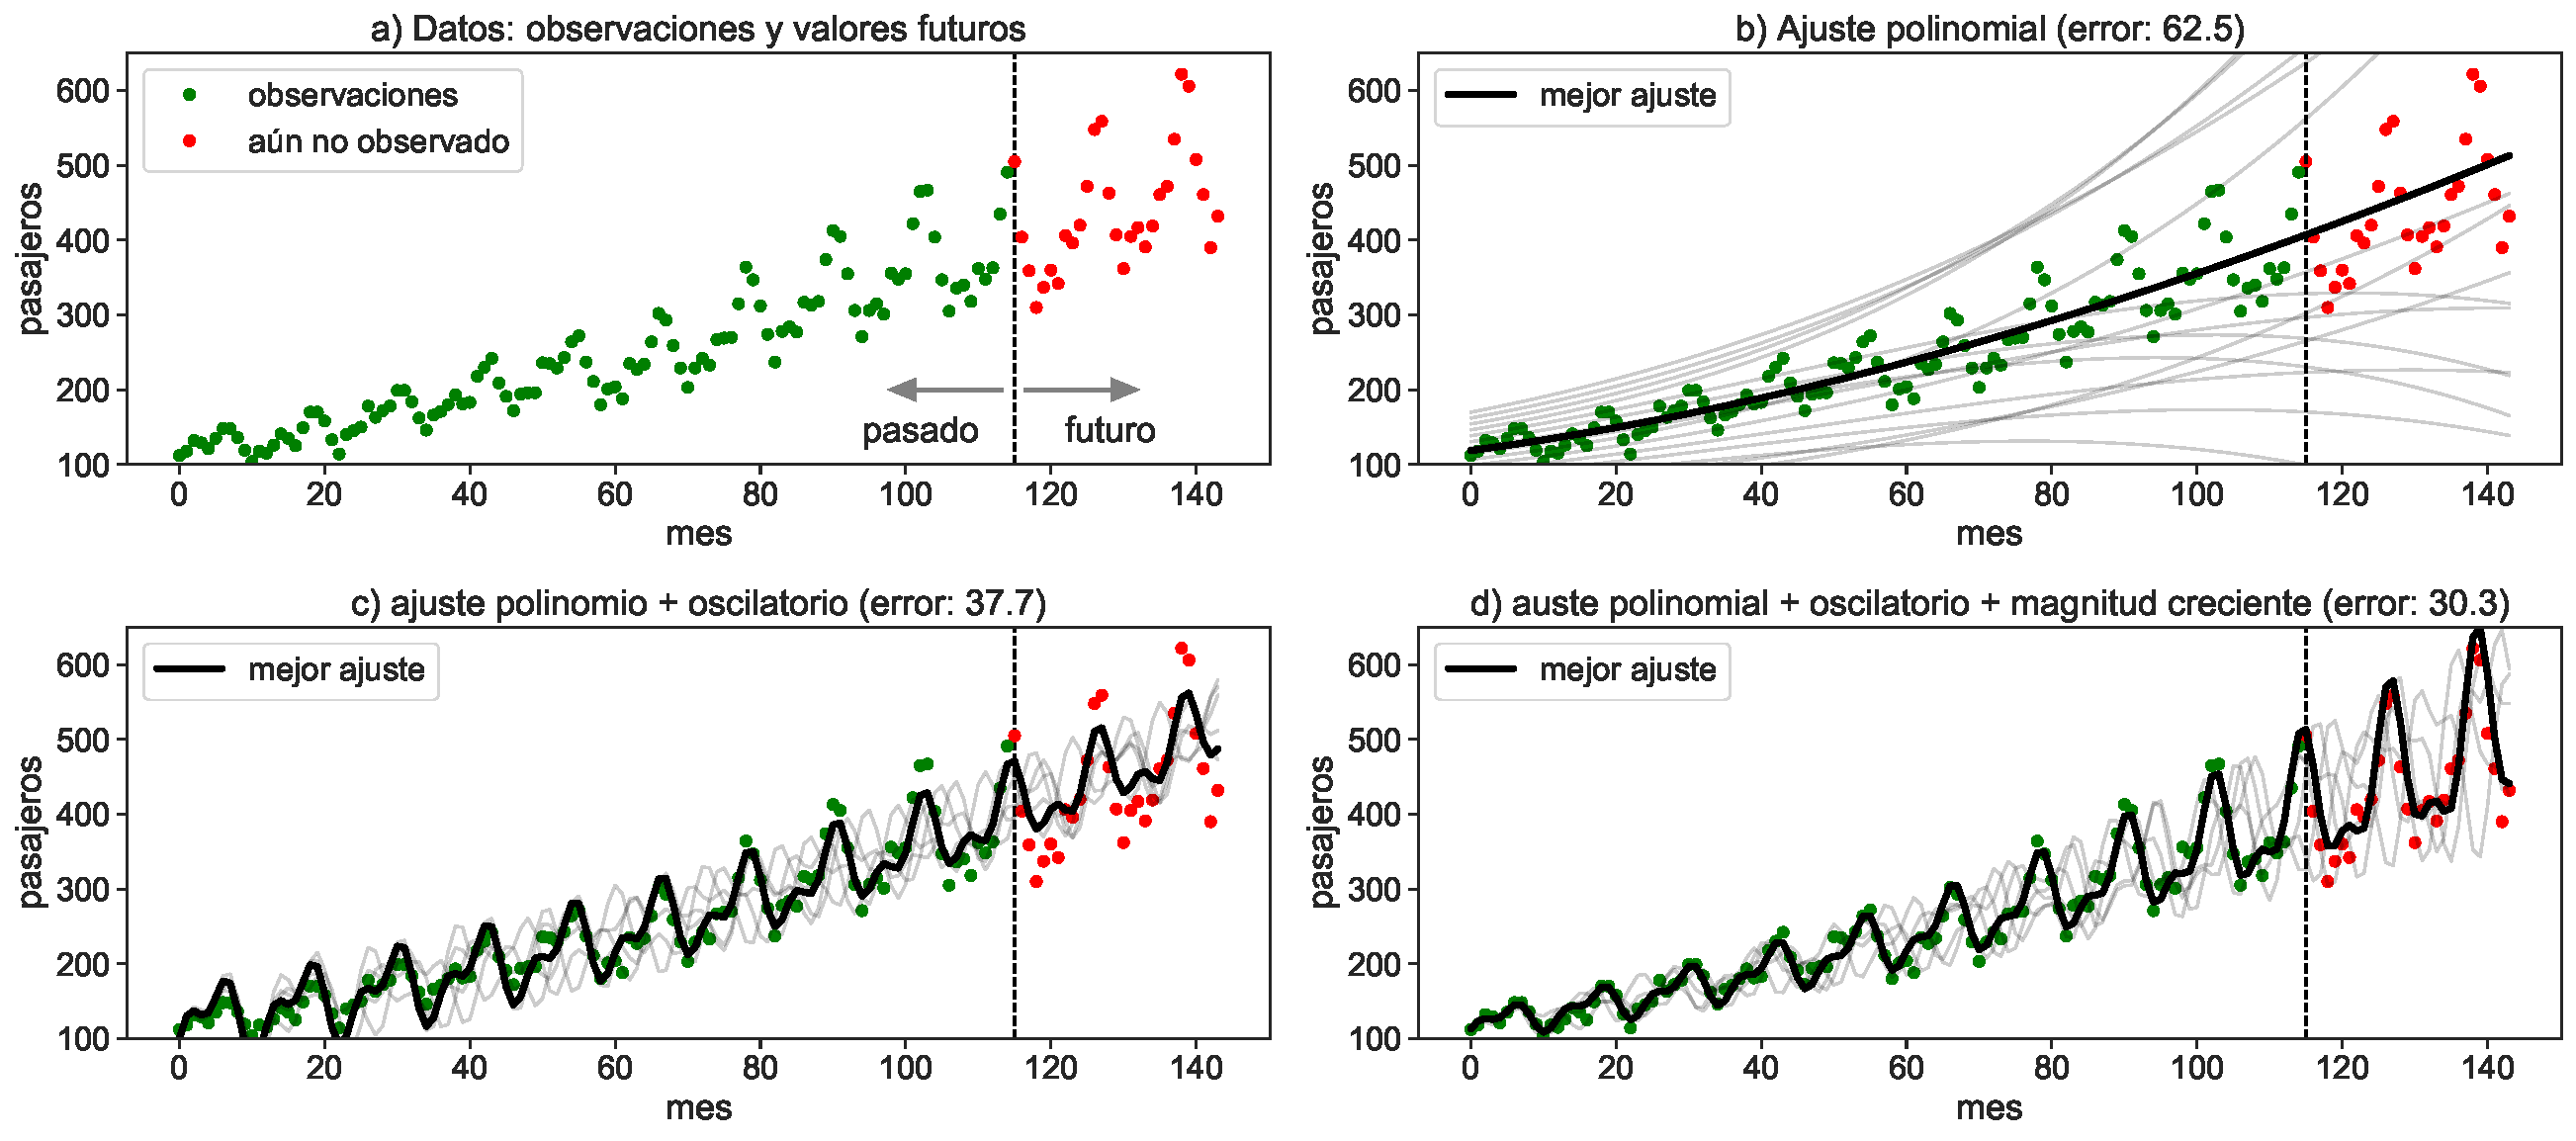
\includegraphics[width=0.9\textwidth, frame]{img/cap1_pasajeros.pdf}
    \caption{Regresión no-linea de cantidad de pasajeros en el tiempo. Arriba-izq: datos de entrenamiento, arriba-der: modelo con componente polinomial, abajo-izq: modelo con componentes polinomial y oscilatoria (amplitud fija), abajo-der: modelo con componentes polinomial y oscilatoria (amplitud creciente).}
    \label{fig:pasajeros}  
\end{figure}
\end{mdframed}




\begin{mdframed}[style=pendiente, frametitle={\center Cosas pendiente}]

\noindent 2) Ejemplo de cómo calcular el gradiente y cómo usar gradiente estocástico

\noindent 3) Discutir el calculo, análisis y muestreo de la posterior 

\noindent 4) Breve mención de variables latentes y casos no-tratables 


\end{mdframed}











